\documentclass{article}

\usepackage[margin=1in]{geometry}
\usepackage{amsmath}
\usepackage{amssymb}
\usepackage{amsthm}
\usepackage{graphicx}
\usepackage{listing}
\usepackage{geometry}
\theoremstyle{definition}
\newtheorem{definition}{Definition}[section]
 \geometry{top=1.75in,left=1.75in,bottom=1.75in,right=1.75in}
\title{Braid Group Cryptography}
\author{
  Madsen, Reese\\
  \texttt{madsenar@clarkson.edu}
  \and
  Pawlaczyk, Tyler\\
  \texttt{pawlactb@clarkson.edu}
   \and
  Klee, Bryan\\
  \texttt{kleebm@clarkson.edu}
}
\date{\today}


\begin{document}

	\maketitle

	\begin{abstract}
	\textbf{Write abstract after paper is done.}
	\end{abstract}
	\newpage
	\section{Braids}
	In this section we will explain the mathematics behind a braid group. A braid group has braids as the set and concatenation as the group operation written as $<B_n,||>$ where $n$ is the number of strands and 

\begin{definition} 
$B_n=\{\sigma_1,...,\sigma_{n-1}:\sigma_i\sigma_j\sigma_i=\sigma_j\sigma_i\sigma_j\ \textrm{if}\ |i-j|=1\ \textrm{and}\ \sigma_i\sigma_j=\sigma_j\sigma_i\ \textrm{if}\ |i-j|>1\}$
\end{definition}
 
A braid group is infinite and nonabelian meaning that the elements do not commute such that:
$a,b \in B_n: \ ab\neq ba$. Note that for $n$ strands there are $n-1$ generators represented by $\sigma$. A braid is the concatenation of generators. A positive generator, $\sigma_i^+$, corresponds to crossing left over right and a negative generator corresponds to crossing right over left, $\sigma_i^-$. 

\begin{figure}[hbp!]
\centering
  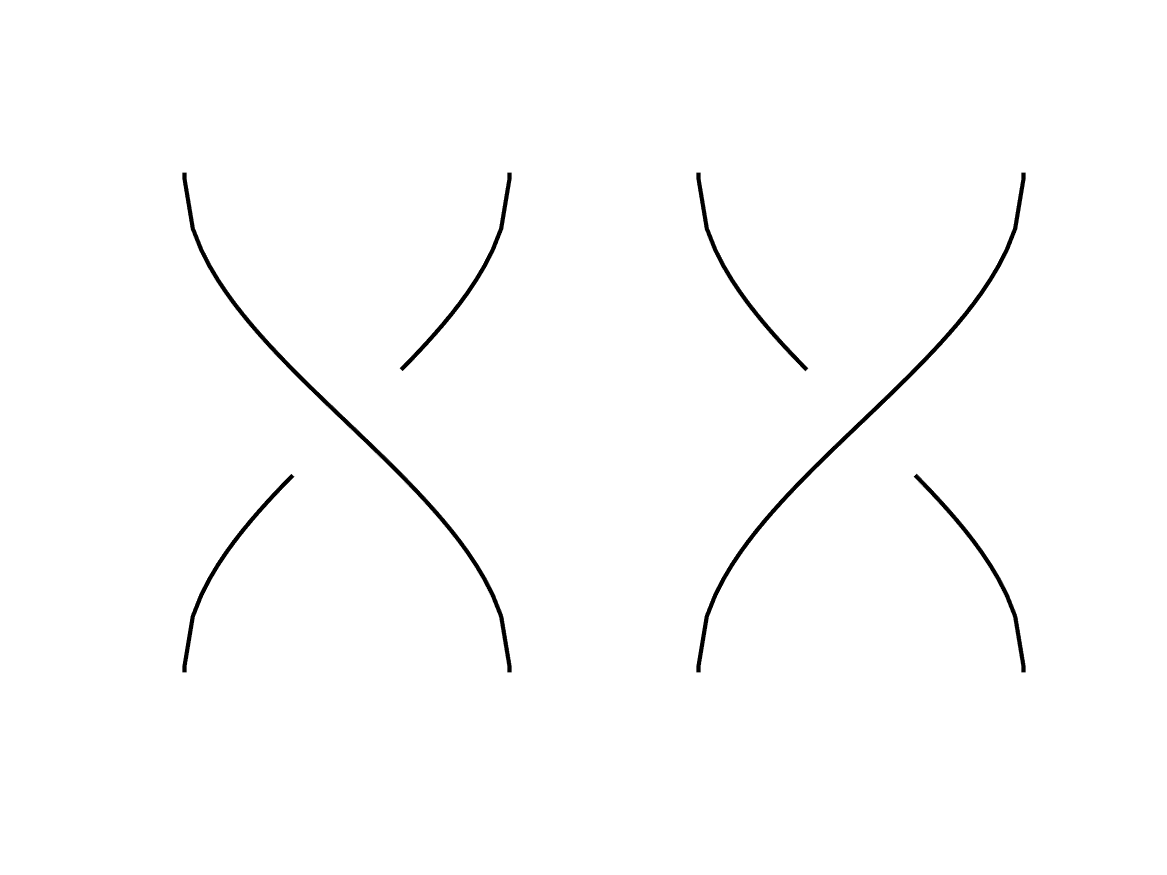
\includegraphics[width=0.2\linewidth]{./Pictures/gen_pos_neg.png}
  \caption{$\sigma_i^+$,$\sigma_i^-$}\label{fig:graph}
\end{figure}

The first rule for braid groups written in the definition states that you are allowed to swap the generators as long as the distance between the generators is one lane apart. The second rule states that as long as the generators do not share a common strand you are allowed to commute them. These can be visualized below:

\begin{figure}[hbp!]
\centering
  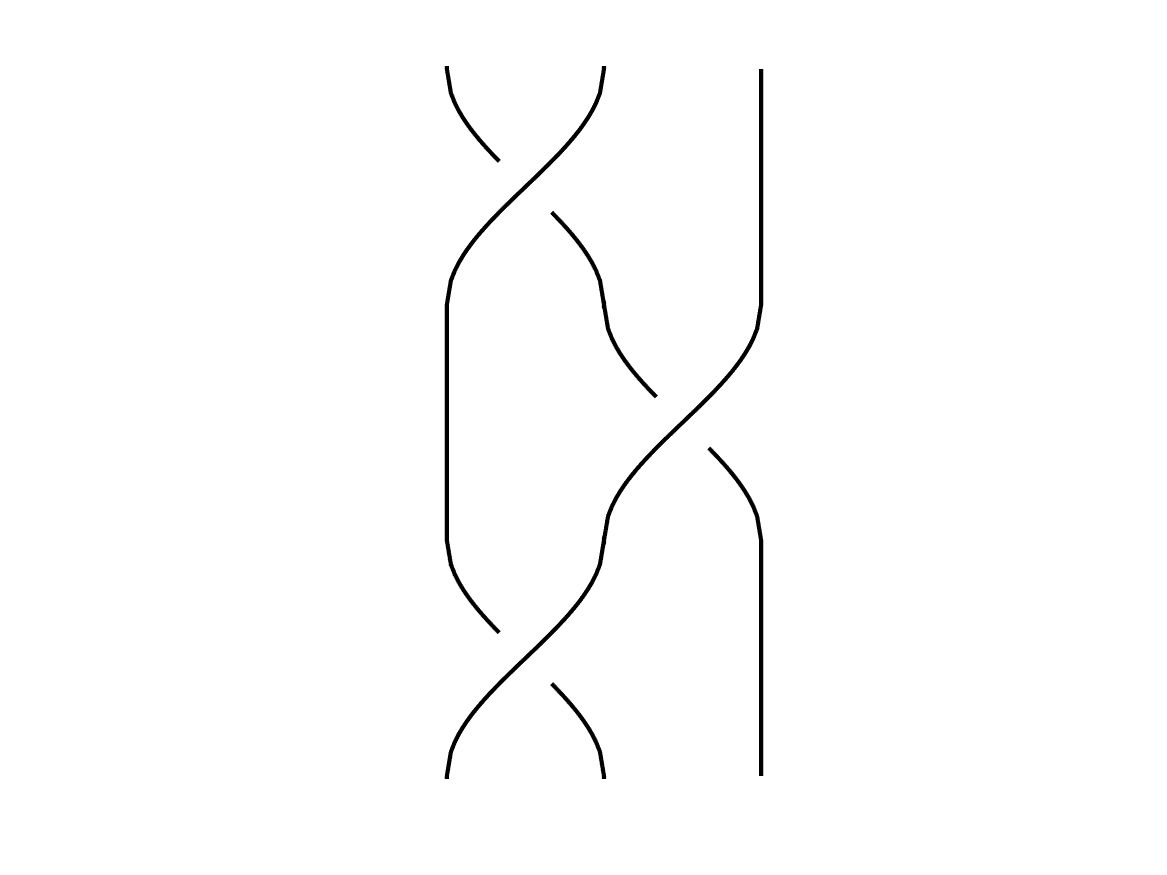
\includegraphics[width=0.2\linewidth]{./Pictures/crisscross_1.png}
   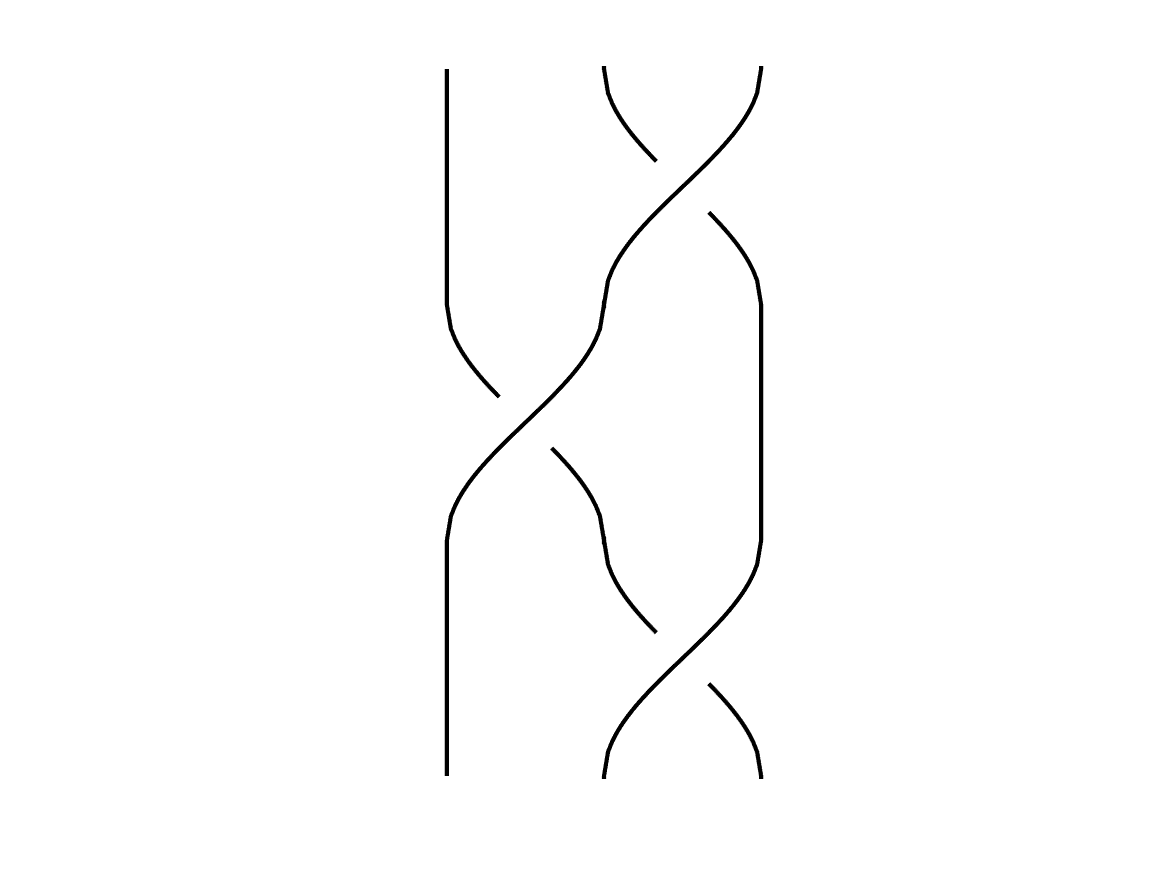
\includegraphics[width=0.2\linewidth]{./Pictures/crisscross_2.png}
  \caption{$\sigma_1\sigma_2\sigma_1=\sigma_2\sigma_1\sigma_2\ \textrm{if}\ |2-1|=1$}\label{fig:graph}
\end{figure}

\begin{figure}[hbp!]
\centering
  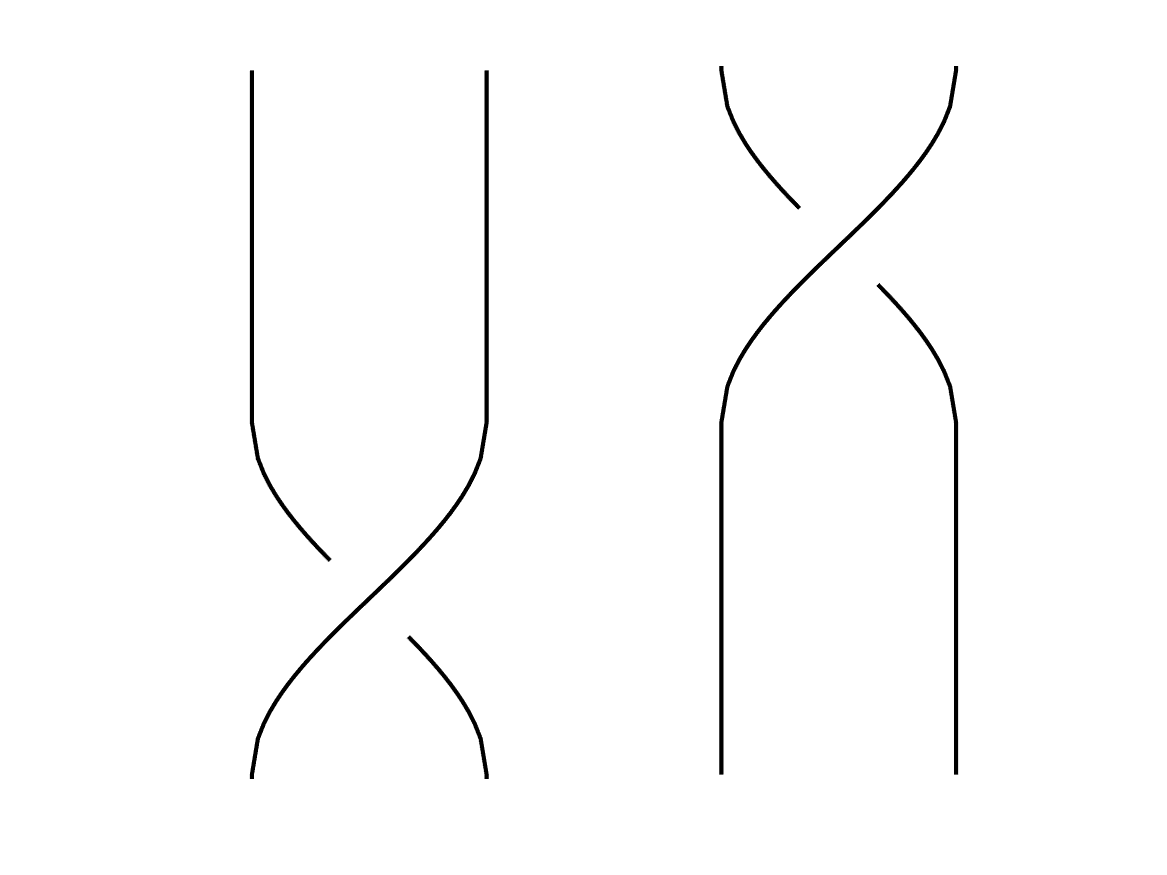
\includegraphics[width=0.2\linewidth]{./Pictures/commute_1.png}
  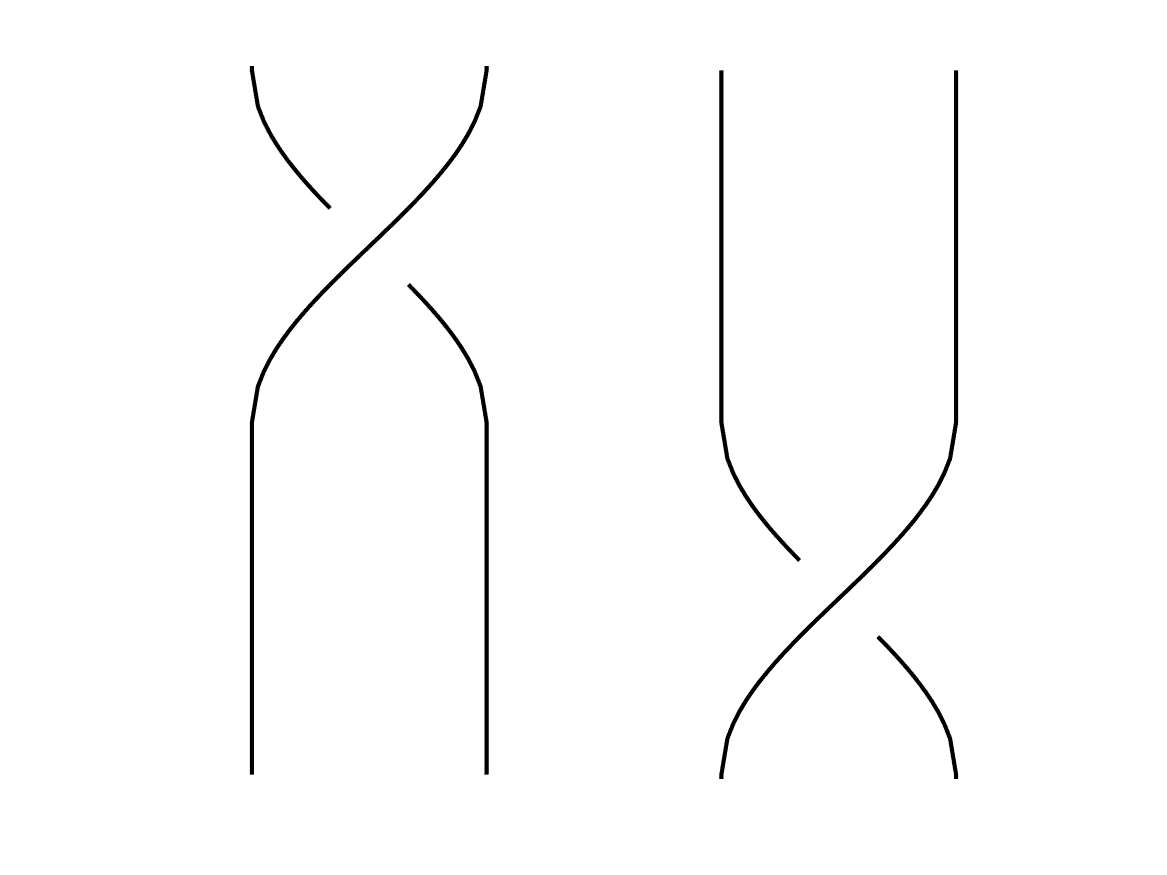
\includegraphics[width=0.2\linewidth]{./Pictures/commute_2.png}
  \caption{$\sigma_1\sigma_3=\sigma_3\sigma_1\ \textrm{if}\ |3-1|>1$}\label{fig:graph}
\end{figure}

For example the braid $b \in B_3: \ b=\sigma_2^+ \sigma_1^+ \sigma_2^- \sigma_1^-$ is the following:
	
	\begin{figure}[hbp!]
\centering
  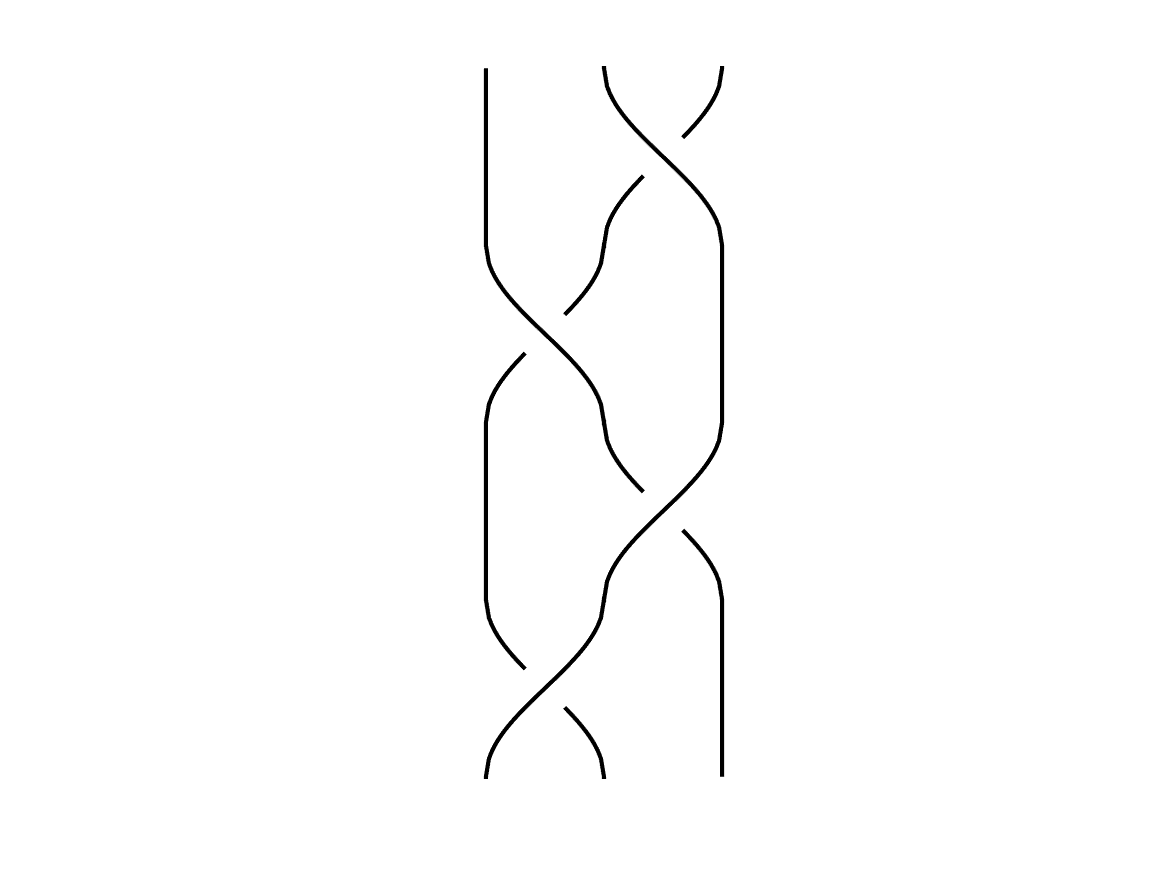
\includegraphics[width=0.2\linewidth]{./Pictures/example_braid.png}
\end{figure}
	
	
\section{Braids as Permutations}
	There is no unique way to write a braid as a concatenation of generators. There is no unique form because you can simply use the rules of the braid group to switch generators around. Therefore there is a connection defined between braid groups and permutation groups so that we can define a uniqueness. There exists a endomorphism:
	$ \phi: B_n \rightarrow \Sigma_n$.
	$\sigma_i $ represents the switch of the i-th strand with the (i+1) strand. 
	Denote the permutation by $\pi \in \Sigma_n, \pi(i)=b_i$. The trick is to then draw straight lines for the permutations on the braid diagram. For example the permutation $\pi=(1 2 3 4)\rightarrow(4 2 1 3)$ maps the 1st strand to the 4th strand and so forth. This corresponds to the following braid $A=\sigma_1 \sigma_2 \sigma_1 \sigma_3$. The fundamental braid $\Delta_n=(\sigma_1...\sigma_{n-1})(\sigma_1 ... \sigma_{n-2})...\sigma_1 $ corresponds to the permutation $\Omega_n=n(n-1),...,(2)(1)=n!$. Now we can define the left canonical form which is used for a unique representation on braids to be utilized in the crypto system.
	
	\begin{definition}	
	For any $w \in B_n$ $\exists$ a unique representation called the left canonical form.
	\\$w = \Delta^u A_1 A_2 ... A_l, u \in Z', A \in \Sigma_n \backslash \{ e, \Delta \} $
	$\text{where } A_i A_{i+1} \text{is left weighted for } 1 \leq i \leq l - 1.$
	\end{definition}
	
	The braids for the crypto system are all in left canonical form for the remainder of the paper. 
	 
	\section{Hard problem associated with braids.}
	As we have seen in RSA and El-Gamal there are associated hard problems with these crypto systems. For RSA there is the factoring problem where for:
	
	\begin{itemize}
		\item p,q \text{are $2$ distinct k-bit primes.}
		\item n=pq 
		\item \text{Multiplying is computationally easy while the inverse function, factoring, is computationally hard.} 
	\end{itemize}

Similarly El-Gamal has the discrete logarithm which is the associated computationally hard problem. 
For braid group cryptography there are several computationally hard problems. One in particular that is widely used is the conjugacy search problem. Conjugacy is defined as:
\begin{definition} 
$G-\text{group. } a,x,y \in G. \text{ If }y=axa^{-1},\text{ then }y \text{ is } conjugate \text{ to }x \text{ via }a.$
\end{definition}

\noindent \textbf{Conjugacy Search Problem:} \\ $\textbf{Given }x,y \in B_n \text{ such that }y=axa^{-1} \text{ for some }a \in B_n. \\ \textbf{Find }b \in B_n \text{ such that }y=b^{-1}xb.$
\\ \\
In Matlab there is a library called Braidlab that utilizes braids and can compute various functions on braids and generators. To represent braids in Matlab a braid $b=\sigma_1^+\sigma_2^-$ would be written as $b=[1 -2]$. Conjugacy is defined as a method for braids called \textbf{conjtest}. The inputs for conjtest are two braids. The method returns true if the braids are conjugate as well as providing the conjugating braid. There are several types of conjugacy search problems and one we will focus on is the Diffie-Hellman type generalized conjugacy search problem. First we need to define $2$ commuting subgroups of $B_n$. 


\begin{definition}
$LB_n,UB_n < B_n. \\ LB_n=\{ \sigma_1,...,\sigma_{[n/2]-1}  \}, UB_n=\{ \sigma_{[n/2]+1},...,\sigma_{n-1}  \} $
\end{definition}

We know use the fact by definition of a braid group that generators commute if and only if the generators do not share a common strand. Since the $\sigma_{n/2}$ generator is missing, elements in each subgroup will commute with each other such that: $a \in LB_n, b \in UB_n, ab=ba$. We can know look at the Diffie-Hellman generalized conjugacy search problem.
\\ \\
\textbf{Diffie-Hellman type Generalized Conjugacy Search Problem:} \\ $\textbf{Given }x,y_A, y_B \in B_n \text{ such that }y_A=axa^{-1} \text{ and } y_B=bxb^{-1} \text{ for some }a \in LB_n \text{ and }b \in UB_n. \\ \textbf{Find }by_Ab^{-1}=ay_Ba^{-1}=abxb^{-1}a^{-1}$

This takes advantage of the fact that we commute $a$ and $b$ which results in the following: $abxb^{-1}a^{-1}=baxa^{-1}b^{-1}$ so both Alice and Bob can decode the message. This problem is used for the key agreement between Alice and Bob.

\section{Background Info and Literature}
\textbf{Include information on what has been done. Talk about state of the art new ideas in braid group cryptography.}

\section{Braid Diffie-Hellman Key Agreement}
First we will discuss the traditional Diffie-Hellman protocol on El-Gamal then look at the key agreement for the braid version Diffie-Hellman. For the traditional Diffie-Hellman agreement the secret keys are $(a,b,g^{ab} \text{mod }p=g^{ab} \text{mod }p)$, and the public keys are $(p,g,g^a \text{mod }p,g^b \text{mod }p)$. 

\begin{definition}
$p \text{ is a prime. } g \text{ is a }\textit{primitive root } \text{of }p \text{ where }g^{p-1}\equiv 1 \text{ mod }p. $
\end{definition}

The next step in the Diffie-Hellman key exchange is for Alice and Bob to select their own keys $a,b \in \mathbb{Z}_p$  secretly and then they send $g^a \text{mod }p$ and $g^b \text{mod }p$ publicly. Then Alice and Bob exponentiate the public keys with their own secret key to obtain the same value. This is dependent on the fact that $ab=ba,  \forall a,b \in \mathbb{Z}_p$. By defining the commuting subgroups of a braid we have the tools needed to define a braid Diffie-Hellman key exchange. 
\\ \\
\textbf{Braid Diffie-Hellman key agreement system.}
\begin{enumerate}

\item \textbf{Preparation Step:} $l=\mid LB_n \mid$ and $r=\mid UB_n \mid$. Pick sufficiently complicated braid such that $x \in B_{l+r}$ which is broadcasted on a public channel. 

\item \textbf{Key Agreement:} 
	 \begin{enumerate}
	 	\item Alice chooses a random secret braid $a \in LB_n$ and sends $y_1=axa^{-1}$ to Bob.
		\item Bob chooses a random secret braid $b \in UB_n$ and sends $y_2=bxb^{-1}$ to Alice.
		\item Alice receives $y_2$ and computes the shared key $K=ay_2a^{-1}=abxb^{-1}a^{-1}$.
		\item Bob receives $y_1$ and computes the shared key $K=by_1b^{-1}=baxa^{-1}b^{-1}$.
	 \end{enumerate}
\item Therefore since for $a \in LB_n$ and $b \in UB_n$, $ab=ba$. Then
\begin{centering}
$ay_2a^{-1}=a(bxb^{-1})a^{-1}=b(axa^{-1})b^{-1}=by_1b^{-1}$. This implies that Alice and Bob both have the same shared braid.
\end{centering}
\end{enumerate}

\section{Algorithm Analysis}


\section{Future Direction and New Ideas}

In the braids as permutation section we mentioned that we can represent the generators of a braid as a permutation group. What about other ways to represent a braid concisely? It turns out that you can also represent generators as matrices using Dynnikov coordinates and the max-plus semiring. The Dynnikov coordinate space is $C_n=\mathbb{R}^{2n-4} \backslash \{0\}$ where $n$ is the number of strands. The idea is to represent generators by looking at how the action of the generator stretches or rotates a given vector. Therefore you can represent each generator by a matrix. This calculation is done using the max-plus semiring. We use this semiring due to the fact that it helps with computation and notation. 

\begin{definition}
The max-semiring $(\mathbb{R},\text{max},+)$ has the maximum function $\text{max}(a,b)$ as the additive operation, and the addition operation $a+b$ as the multiplicative operation. It is a semiring due to the fact that there is not an additive inverse.
\end{definition}

\noindent Here is an example that shows how to represent a generator as a matrix: For $n=3$, the possible generators are $\sigma_1^+, \sigma_1^-, \sigma_2^+, \sigma_2^-$. Also the input vector comes from the Dynnikov coordinate space: $x \in \mathbb{R}^{2n-4} = \mathbb{R}^{2(3)-4}$. For the generator $\sigma_1^+ (a,b)=(a',b')$ where 
\\ \\
$[a+b]=\text{max}(a,b), [ab]=a+b, [a/b]=a-b, \text{ and } [1]=0. \\ \\ a'=[\frac{ab}{a+1+b}], b'=[\frac{1+b}{a}],   \\ \text{ If } 0<a<b , \text{then } \sigma_1^+ (a,b)=
\begin{bmatrix}
1 & 0\\
-1 & 1
\end{bmatrix} $. We want to compare the $a$ and $b$ and obtain different matrices for several cases. Since we can represent generators as matrices we can use this to our advantage due to the fact that computers work with arrays and matrices well! This is a proposed alternative method to representing braids as permutation groups. Using results in linear algebra perhaps a more efficient system may be worth trying. 

The creation of braids in the crypto system is dependent on generating random braids. This is done by generating random permutations of the braids then turning them into left canonical form so that the braids are unique. The random generation is done by using an oracle which helps with decision making. Here we propose a new method of generating random braids using brownian motion. Brownian motion is defined as the way particles move and bump against each other in a fluid. This movement is stochastic which can help us in generating random braids. The way to represent brownian motion is by using differential equations. Here is the stochastic differential equation: $dX_t=F(t,X_t) dt+G(t,X_t) dW_t$ where $F$ is the vector of drifting rates, $G$ is the matrix of volatility rates, $t$ is time, $X_t$ is the state vector, and $dW_t$ is the vector of possible correlated drift and volatility rates. The trajectories in the braid will follow this random walk and then cross depending on how stochastic the movement is. For example if the volatility rates were very low then the trajectories would not move around each other very much which would result in not many crossings of the trajectories. Therefore choosing the drift and volatility rates are very important to be able to obtain a significant braid. Once a sufficient braid is obtained from these random trajectories, the braid will be inherently random due to the fact that brownian motion is stochastic. After the random braids are obtained they can be changed into left canonical form which would be used for the cryptosystem. 



\begin{thebibliography}{9}

\bibitem{braid_groups_intro} 
Parvez Anandam. 
\textit{Introduction to Braid Group Cryptography}. 
March 7, 2006.
 
\bibitem{new_public_crypto} 
Ki Hyoung Ko, Sang Jin Lee, Jung Hee Cheon, Jae Woo Han, Ju-sung Kang, Choonsik Park.
\textit{New Public-key Cryptosystem Using Braid Groups}.
Korea Advanced Institute of Science and Technology, Brown University, Electronics and Telecommunications Research Institute. 

\bibitem{braid_group_crypto}
David Garber.
\textit{Braid Group Cryptography}.
Department of Applied Mathematics, Holon Institute of Technology. 
 
 \bibitem{new_directions}
Whitfield Diffie, Martin Hellman. (November 1976)
\textit{New Directions in Cryptography}.
IEEE Transactions on Information Theory.


\bibitem{dynn_coordinates}
Toby Hall, S. Oyku Yurttas.
\textit{On the Topological Entropy of Families of Braids}.

\bibitem{imp_braid_groups}
Jae Choon Cha, Ki Hyoung Ko, Sang Jin Lee, Jung Hee Cheon, Jae Woo Han.
\textit{An Efficient Implementation of Braid Groups}.

\bibitem{braidlab}
Jean-Luc Thiffeault, Marko Budisic.
\textit{Braidlab: A Software Package for Braids and Loops}.

\end{thebibliography}






	
\end{document}